%%%%%%%%%%%%%%%%%%%%%%%%%%%%%%%%%%%
%This is the LaTeX COMMUNICATION template for RSC journals
%Copyright The Royal Society of Chemistry 2016
%%%%%%%%%%%%%%%%%%%%%%%%%%%%%%%%%%%

\documentclass[twoside,twocolumn,9pt]{article}
\usepackage{extsizes}
\usepackage[super,sort&compress,comma]{natbib} 
\usepackage[version=3]{mhchem}
\usepackage[left=1.5cm, right=1.5cm, top=1.785cm, bottom=2.0cm]{geometry}
\usepackage{balance}
\usepackage{mathptmx}
\usepackage{sectsty}
\usepackage{graphicx} 
\usepackage{lastpage}
\usepackage[format=plain,justification=justified,singlelinecheck=false,font={stretch=1.125,small,sf},labelfont=bf,labelsep=space]{caption}
\usepackage{float}
\usepackage{fancyhdr}
\usepackage{fnpos}
\usepackage[english]{babel}
\addto{\captionsenglish}{%
  \renewcommand{\refname}{Notes and references}
}
\usepackage{array}
\usepackage{droidsans}
\usepackage{charter}
\usepackage[T1]{fontenc}
\usepackage[usenames,dvipsnames]{xcolor}
\usepackage{setspace}
\usepackage[compact]{titlesec}
\usepackage[hidelinks]{hyperref}
%%%Please don't disable any packages in the preamble, as this may cause the template to display incorrectly.%%%


% xr to cross reference files
\usepackage{xr}
\externaldocument{SI}

% https://stackoverflow.com/questions/1856189/fullpage-picture-in-two-column-layout
\usepackage{dblfloatfix}

\usepackage{amsmath, amssymb}

% Custom commands ---------------------------
\newcommand{\kcal}{kcal mol$^{-1}$}
\graphicspath{ {figures/} }


% ------------------------------------------------

%\usepackage{epstopdf}%This line makes .eps figures into .pdf - please comment out if not required.

\definecolor{cream}{RGB}{222,217,201}

\begin{document}

\pagestyle{fancy}
\thispagestyle{plain}
\fancypagestyle{plain}{
%%%HEADER%%%
\renewcommand{\headrulewidth}{0pt}
}
%%%END OF HEADER%%%

%%%PAGE SETUP - Please do not change any commands within this section%%%
\makeFNbottom
\makeatletter
\renewcommand\LARGE{\@setfontsize\LARGE{15pt}{17}}
\renewcommand\Large{\@setfontsize\Large{12pt}{14}}
\renewcommand\large{\@setfontsize\large{10pt}{12}}
\renewcommand\footnotesize{\@setfontsize\footnotesize{7pt}{10}}
\renewcommand\scriptsize{\@setfontsize\scriptsize{7pt}{7}}
\makeatother

\renewcommand{\thefootnote}{\fnsymbol{footnote}}
\renewcommand\footnoterule{\vspace*{1pt}% 
\color{cream}\hrule width 3.5in height 0.4pt \color{black} \vspace*{5pt}} 
\setcounter{secnumdepth}{5}

\makeatletter 
\renewcommand\@biblabel[1]{#1}            
\renewcommand\@makefntext[1]% 
{\noindent\makebox[0pt][r]{\@thefnmark\,}#1}
\makeatother 
\renewcommand{\figurename}{\small{Fig.}~}
\sectionfont{\sffamily\Large}
\subsectionfont{\normalsize}
\subsubsectionfont{\bf}
\setstretch{1.125} %In particular, please do not alter this line.
\setlength{\skip\footins}{0.8cm}
\setlength{\footnotesep}{0.25cm}
\setlength{\jot}{10pt}
\titlespacing*{\section}{0pt}{4pt}{4pt}
\titlespacing*{\subsection}{0pt}{15pt}{1pt}
%%%END OF PAGE SETUP%%%

%%%FOOTER%%%
\fancyfoot{}
\fancyfoot[LO,RE]{\vspace{-7.1pt}
\includegraphics[height=9pt]{head_foot/LF}}
\fancyfoot[CO]{\vspace{-7.1pt}\hspace{13.2cm}
\includegraphics{head_foot/RF}}
\fancyfoot[CE]{\vspace{-7.2pt}\hspace{-14.2cm}
\includegraphics{head_foot/RF}}
\fancyfoot[RO]{\footnotesize{\sffamily{1--\pageref{LastPage} ~\textbar  \hspace{2pt}\thepage}}}
\fancyfoot[LE]{\footnotesize{\sffamily{\thepage~\textbar\hspace{3.45cm} 1--\pageref{LastPage}}}}
\fancyhead{}
\renewcommand{\headrulewidth}{0pt} 
\renewcommand{\footrulewidth}{0pt}
\setlength{\arrayrulewidth}{1pt}
\setlength{\columnsep}{6.5mm}
\setlength\bibsep{1pt}
%%%END OF FOOTER%%%

%%%FIGURE SETUP - please do not change any commands within this section%%%
\makeatletter 
\newlength{\figrulesep} 
\setlength{\figrulesep}{0.5\textfloatsep} 

\newcommand{\topfigrule}{\vspace*{-1pt}% 
\noindent{\color{cream}\rule[-\figrulesep]{\columnwidth}{1.5pt}} }

\newcommand{\botfigrule}{\vspace*{-2pt}% 
\noindent{\color{cream}\rule[\figrulesep]{\columnwidth}{1.5pt}} }

\newcommand{\dblfigrule}{\vspace*{-1pt}% 
\noindent{\color{cream}\rule[-\figrulesep]{\textwidth}{1.5pt}} }

\makeatother
%%%END OF FIGURE SETUP%%%

%%%TITLE AND AUTHORS%%%
\twocolumn[
  \begin{@twocolumnfalse}
{
\includegraphics[height=30pt]{head_foot/journal_name}\hfill\raisebox{0pt}[0pt][0pt]{
\includegraphics[height=55pt]{head_foot/RSC_LOGO_CMYK}}\\[1ex]

\includegraphics[width=18.5cm]{head_foot/header_bar}}\par
\vspace{1em}
\sffamily
\begin{tabular}{m{4.5cm} p{13.5cm} }


\includegraphics{head_foot/DOI} & \noindent\LARGE{\textbf{Reaction Dynamics of Diels-Alder Reactions from Machine Learned Potentials}} \\%Article title goes here instead of the text "
"
 & \vspace{0.3cm} \\

 & \noindent\large{Tom A. Young,\textit{$^{a}$} Tristan Johnston-Wood,\textit{$^{a}$}, Hanwen Zhang\textit{$^{a}$} and Fernanda Duarte$^\ast$\textit{$^{a}$}} \\%Author names go here instead of "Full name", etc.

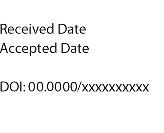
\includegraphics{head_foot/dates} & \\

\end{tabular}

 \end{@twocolumnfalse} \vspace{0.6cm}

  ]
%%%END OF TITLE AND AUTHORS%%%

%%%FONT SETUP - please do not change any commands within this section
\renewcommand*\rmdefault{bch}\normalfont\upshape
\rmfamily
\section*{}
\vspace{-1cm}


%%%FOOTNOTES%%%

\footnotetext{\textit{$^{a}$~Chemical Research Laboratory, South Parks Road, Oxford, OX1 1NQ.}}

%Please use \dag to cite the ESI in the main text of the article.
%If you article does not have ESI please remove the the \dag symbol from the title and the footnotetext below.
\footnotetext{\dag~Electronic Supplementary Information (ESI) available.}
%additional addresses can be cited as above using the lower-case letters, c, d, e... If all authors are from the same address, no letter is required

% \footnotetext{\ddag~Additional footnotes to the title and authors can be included \textit{e.g.}\ `Present address:' or `These authors contributed equally to this work' as above using the symbols: \ddag, \textsection, and \P. Please place the appropriate symbol next to the author's name and include a \texttt{\textbackslash footnotetext} entry in the the correct place in the list.}

%%%END OF FOOTNOTES%%%

%%%ABSTRACT%%%%

\sffamily{\textbf{Machine learned potentials (MLPs) for reactive chemical systems will enable reaction rates to be estimated quickly and accurately. Here, we show that recent advancements in MLP regression methods enable quantum dynamics and umbrella sampling to be performed routinely by leveraging automated fitting and active learning. Product distributions of ambimodal reactions are strongly dependent on the QM method and less so on the type of dynamics propagated. Reaction free energies from umbrella sampling for reactions containing 10s of atoms are obtainable within a day.}}\\

%%%END OF ABSTRACT%%%%

\rmfamily %Please do not remove this line.

%%%MAIN TEXT%%%%

Simulating chemical reactions is essential to developing fundamental understanding and predicting experimental outcomes.\cite{Orr-Ewing2017} Machine learned potentials (MLPs) offer an enticing approach to chemical simulation, enabling the efficient mapping between nuclear configurations and energies ($\boldsymbol{R} \mapsto E$). Moreover, they offer flexibility and systematic improvability, in contrast to classical molecular mechanics (MM).\cite{Behler2016} Propagating quantum dynamics using these forces should afford experimental rate and equilibrium constants in the limit of correct forces and converged sampling. However, despite the development of Gaussian Approximation Potentials (GAPs)\cite{Bartk2010, Deringer2021} and high dimensional neural network potentials (NNPs)\cite{Behler2007} more than 10 years ago, they are still not yet routinely used to simulate chemical reactivity.\cite{Ko2020} Most likely, this is due to the computational and time investment required to train potentials for new systems. 

Training an MLP consists of: (1) developing a training set; (2) hyperparameter optimisation and (3) performing the regression, repeating the process until the desired accuracy is obtained. Automated approaches to training set construction have been developed,\cite{Smith2018, Young2021gap, Miksch2021} but can be limited to small systems or generate huge datasets. These limitations coupled with the time required to perform hyperparameter optimisation (if the MLP is insufficiently accurate) inhibits quickly accessing bespoke MLPs. Furthermore, the required $\gg10^3$ reference evaluations precludes using accurate wavefunction-based quantum methods to evaluate energy and forces without considerable investment.\cite{Smith2019} Exceptions are rare and limited to systems with $\lesssim 10$ atoms.\cite{Young2021gap, Dral2020}

For potentials suitable to simulate chemical reactivity, automated approaches are essential. The energy scale over which the potential must be accurate is larger, necessitating more training data and thus bespoke MLPs. Furthermore, the complex electronic structure around transition states means coupled-cluster (CC) rather than density functional theory (DFT) is often the target surface for quantitative comparison to experiment,\cite{Zhao2005} which in-turn demands data-efficient strategies. 

Here, we show that new MLP methods\cite{Batzner2021, Kovacs2021} can be used to generate accurate potentials for modestly sized reactions ($\sim50$ atoms) in an automated way, and outline some resulting insights. 


\begin{figure*}[tb]
	\centering
	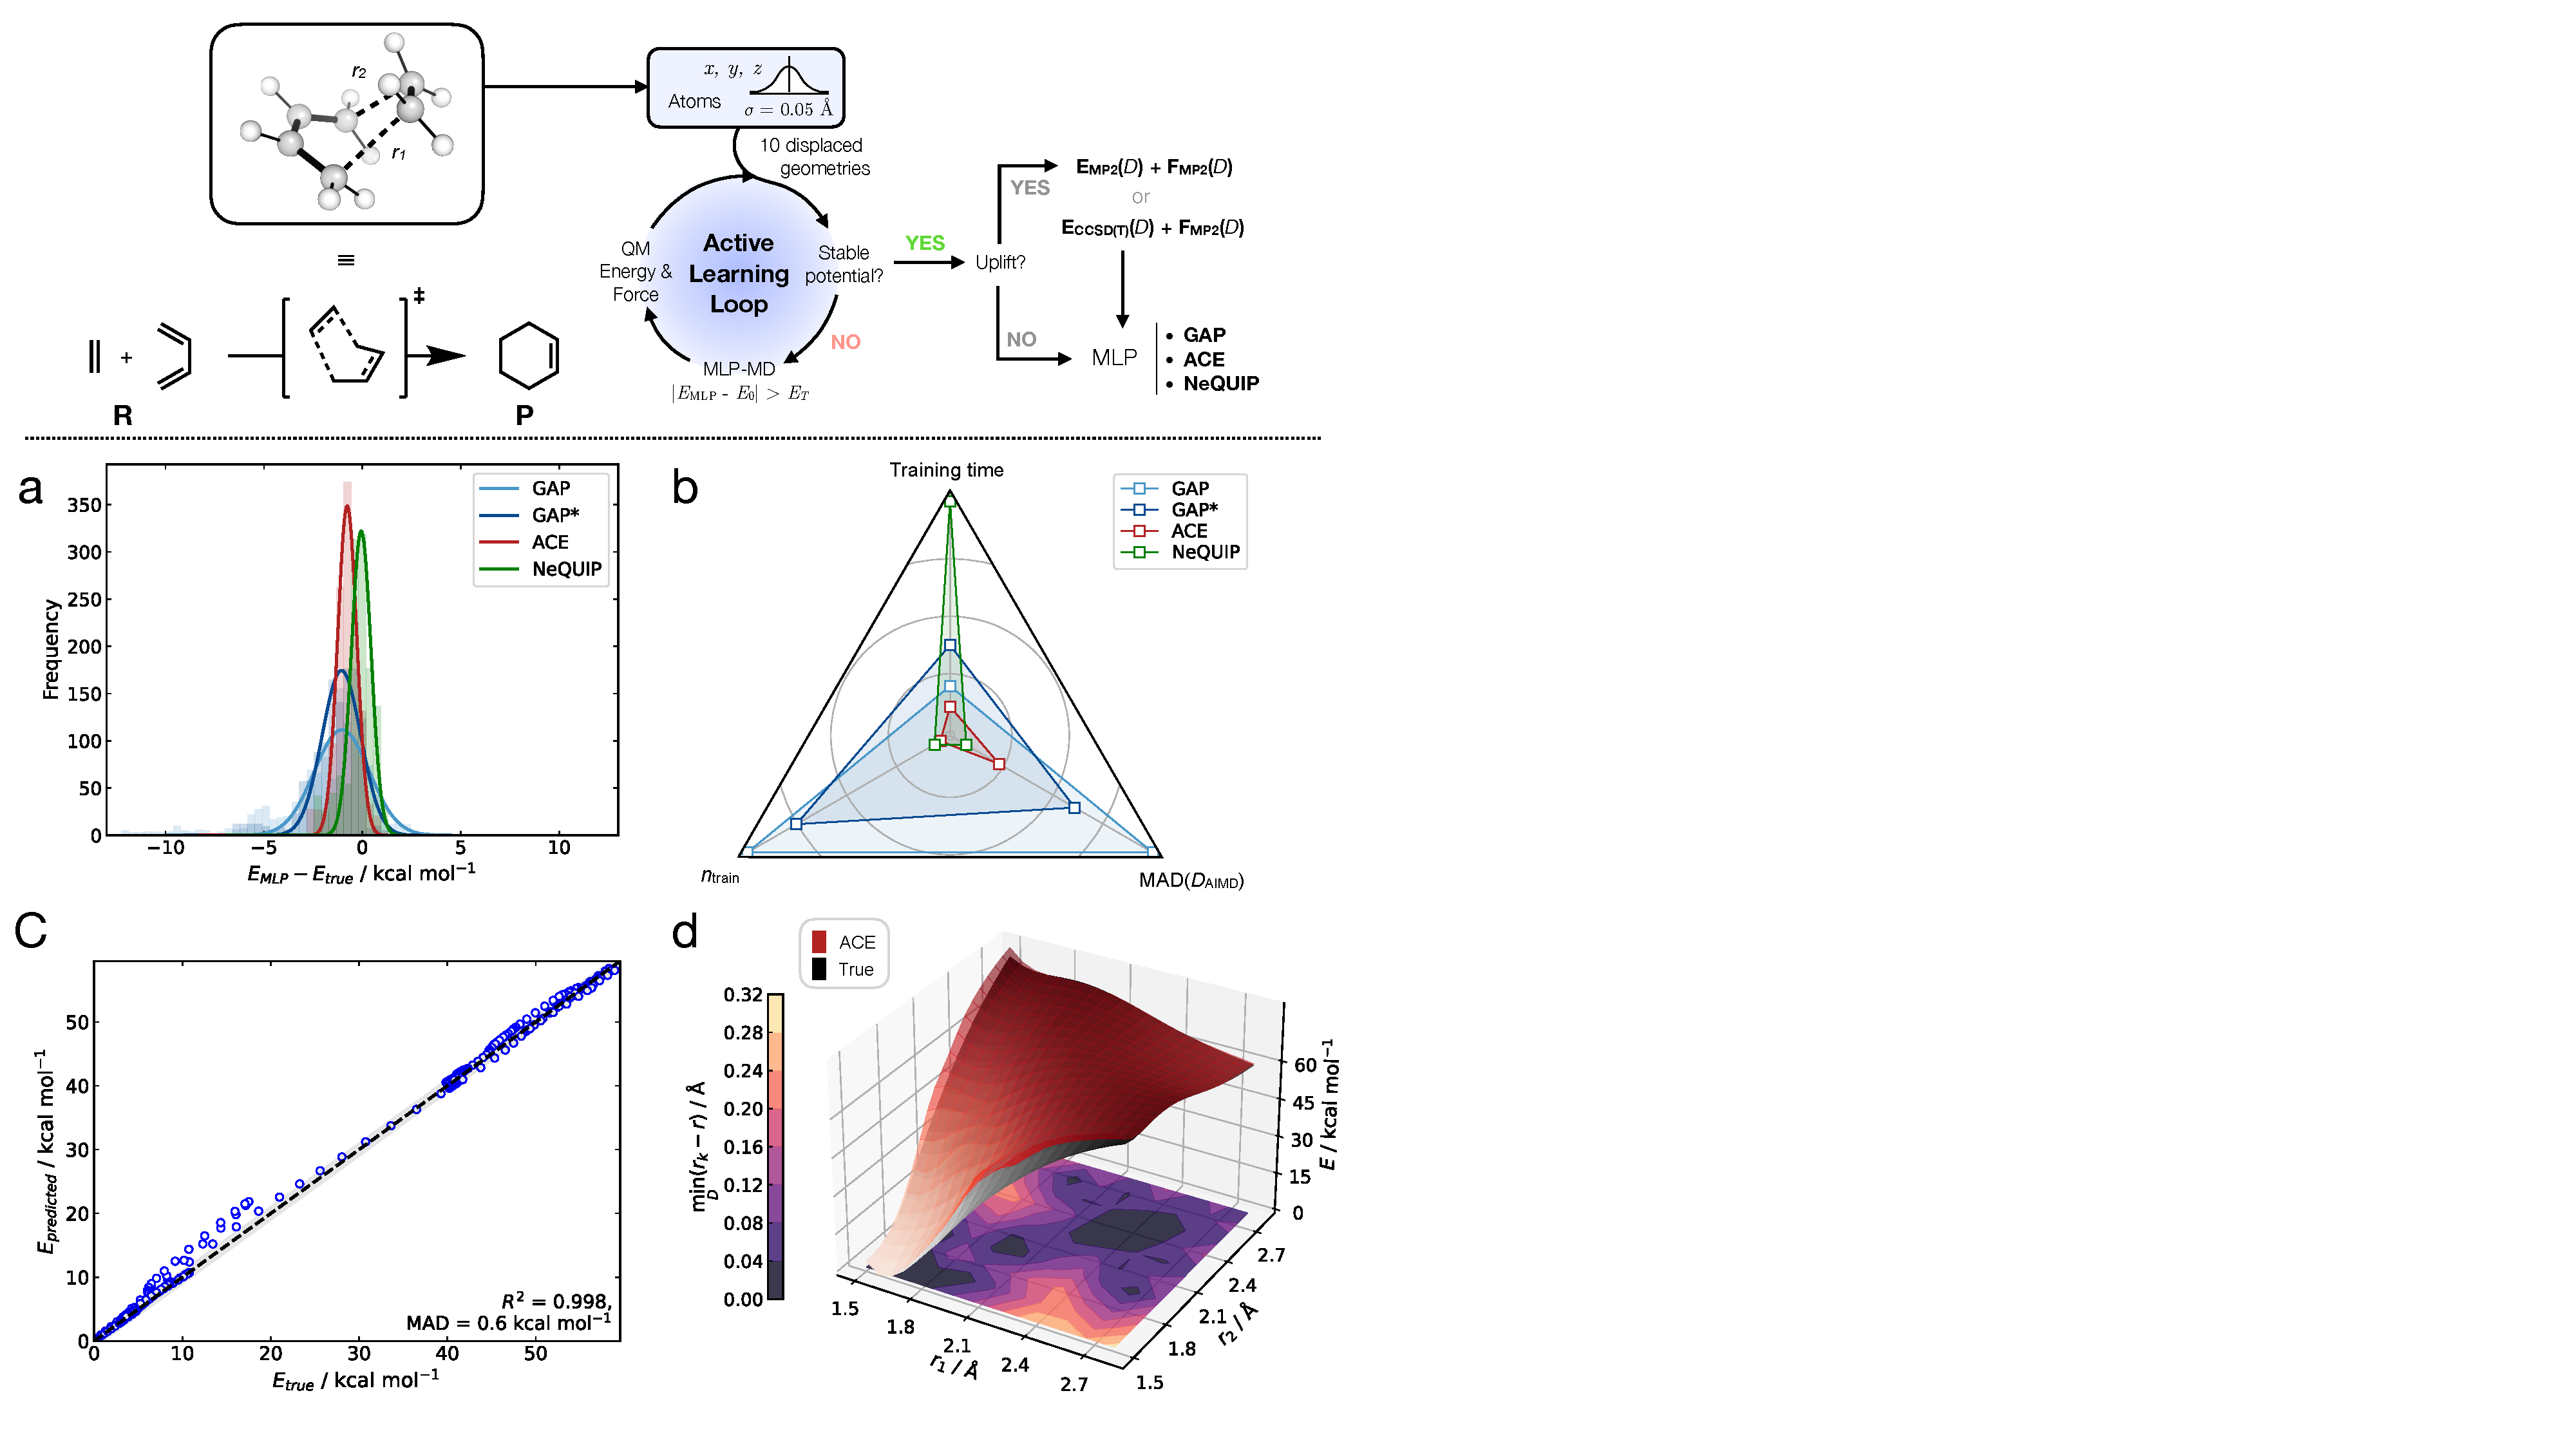
\includegraphics[width=\textwidth]{figX1}
	%\vspace{0.1cm}
	%\hrule
	%\vspace{0.1cm}
	\caption{MLP methods trained on the [4+2] Diels-Alder cycloaddition between ethene and butadiene in the gas phase. GAP* used optimised hyperparameters (see SI §\ref{section::SI_hyperparam_opt_summary}). Training set developed by active learning based on MLP-dynamics with $E_T$ = 2.3 \kcal~(0.1 eV), stable potential defined by the ability to propagate 10 trajectories without finding a configuration $|E_\text{MLP} - E_0| > E_T$. (a) Signed errors on total energies over three trajectories from reactants to products (AIMD, 300K, PBE0/def2-SVP). (b) Comparison of the relative performance between MLP methods on total time, data efficiency (number of training configuration selected, $n_\text{train}$) and total accuracy. (c) Parity plot between MP2/def2-TZVP total energies and ACE predictions on MP2 AIMD trajectories from the TS. ACE trained on DFT selected configurations; energies and forces re-evaluated at MP2. (d) Comparison of the predicted (red) and true PBE0/def2-SVP (black) relaxed 2D surface surrounding the TS. Contour plot represents the ‘closeness’ of the training data to a point in the surface.}
	\label{fig::X1}
\end{figure*}



\begin{figure*}[b]
	\centering
	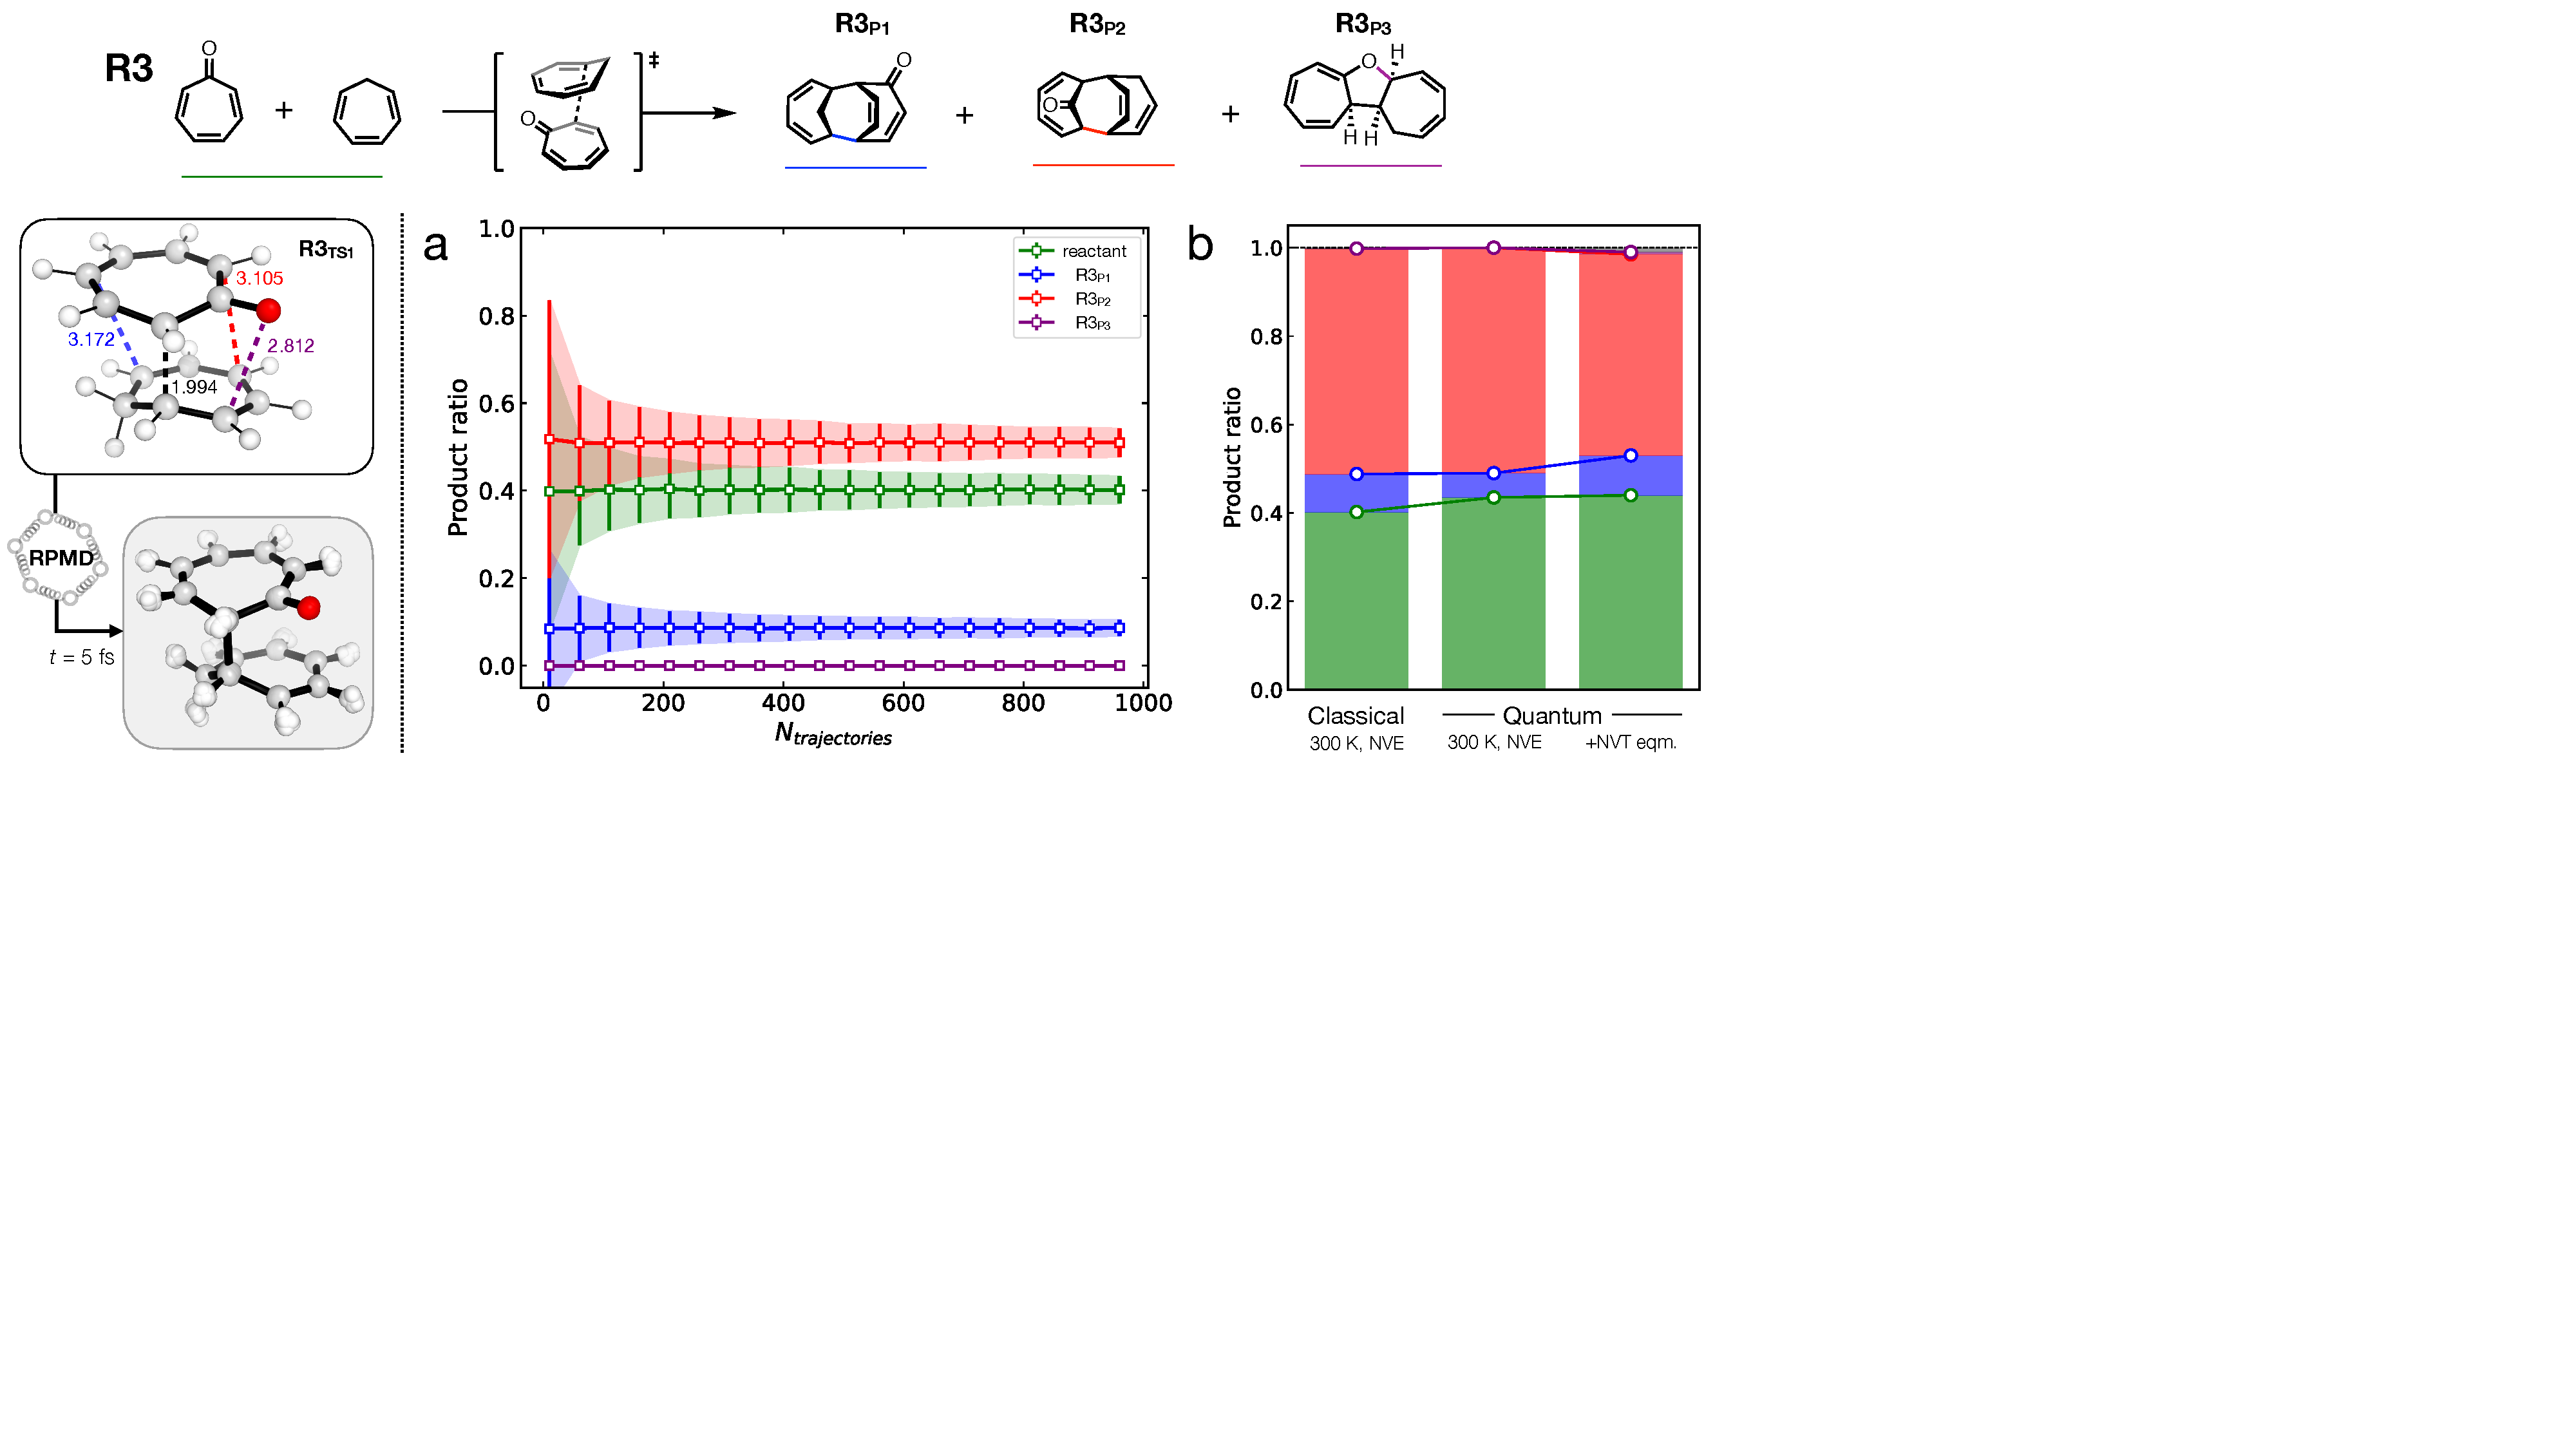
\includegraphics[width=0.85\textwidth]{figX2}
	%\vspace{0.1cm}
	%\hrule
	%\vspace{0.1cm}
	\caption{Product distributions for the reaction between tropone and cycloheptatriene by ACE molecular dynamics simulations initiated from a single TS (top right). ACE potential trained using a standard active learning loop (diff, $E_T$ = 2.3 \kcal~= 0.1 eV, 500 K dynamics) from two TS, such that the training data included all three products. (a) Convergence of the product ratio (e.g. $N_{\rightarrow R3_{P1}} / N_\text{total}$) with number of trajectories propagated. Error is quoted as $2\sigma$, obtained from bootstrapping with resampling (1000 iterations) on the same dataset. Dynamics propagated classically in the NVE ensemble from the TS using initial Boltzmann-sampled velocities for 300 K. (b) Dependence of the product ratio on the type of propagated dynamics ($N_\text{total}$ = 200), including classical MD [as (a)] and ring polymer molecular dynamics (RPMD). RPMD simulations initiated from the TS, or first equilibrated using constrained NVT dynamics (80 fs, harmonic: 4 distances (top left), $k$ = 1 eV \AA${}^{-1}$) then NVE. All NVE simulations performed for 1 ps using a 0.5 fs timestep. Accuracy of the ACE potential trained on PBE0/def2-SVP energies and forces is shown in Fig. \ref{fig::SX33}.}
	\label{fig::X2}
\end{figure*}


\begin{figure*}[b]
	\centering
	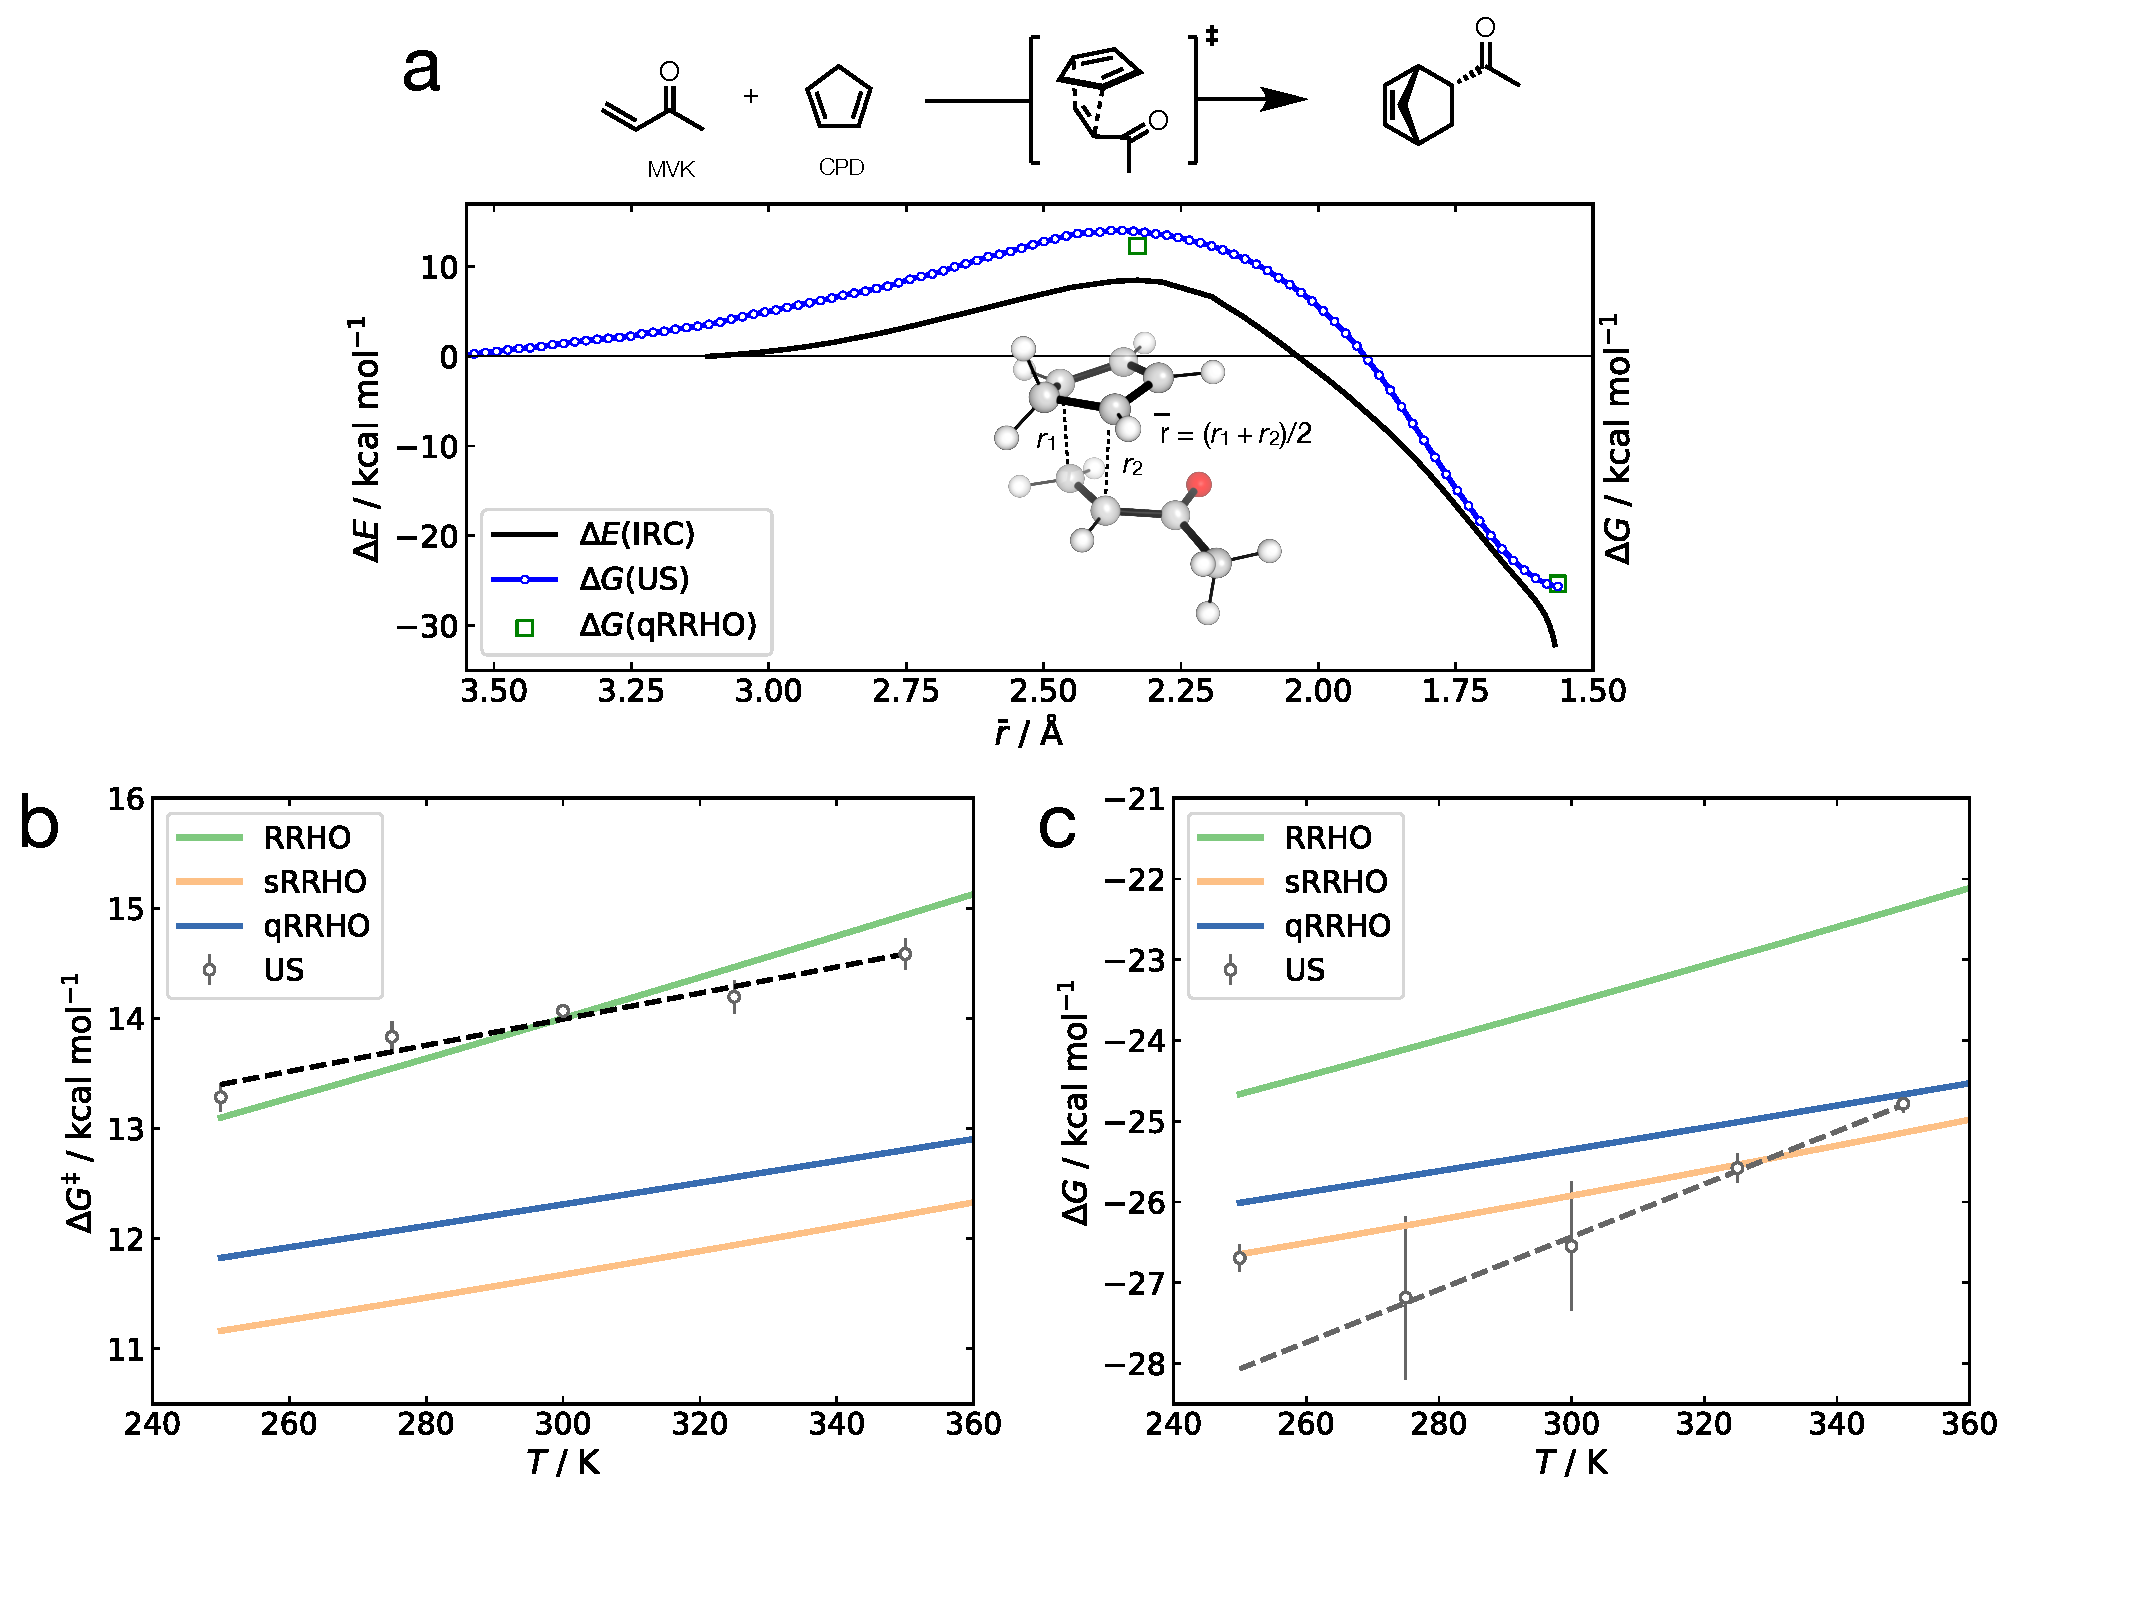
\includegraphics[width=\textwidth]{figX3}
	%\vspace{0.1cm}
	%\hrule
	%\vspace{0.1cm}
	\caption{Reaction and transition state free energies for the reaction between methyl vinyl ketone (MVK) and cyclopentadiene (CPD). (a) Comparison of the intrinsic reaction coordinate energy potential, quasi-rigid rotor harmonic oscillator (qRRHO) and umbrella sampling (US) free energies (300 K). Umbrella sampling performed using a ACE potential trained at the PBE0-D3BJ/def2-SVP level of theory at 500 K from the TS, then 30 windows simulated at the required temperature over the reaction coordinate (average of the forming bonds, $\bar{r}$) for 10 ps. See Fig. \ref{fig::SX34} for umbrella histograms. End point values from optimised structures at the DFT level. (b) Free energy barrier as a function of temperature using different static endpoint and intermediate path methods. sRRHO corresponds to a shifted RRHO treatment of the vibrational entropy where modes $<100$ cm$^{-1}$ are shifted to 100 cm$^{-1}$. Vibrational frequencies calculated at the DFT level from minima. Free energies from classical US are averaged over 5 repeats and the error the standard error of the mean. (c) Reaction free energy change. Simulations as (b).}
	\label{fig::X3}
\end{figure*}

\begin{figure*}[tb]
	\centering
	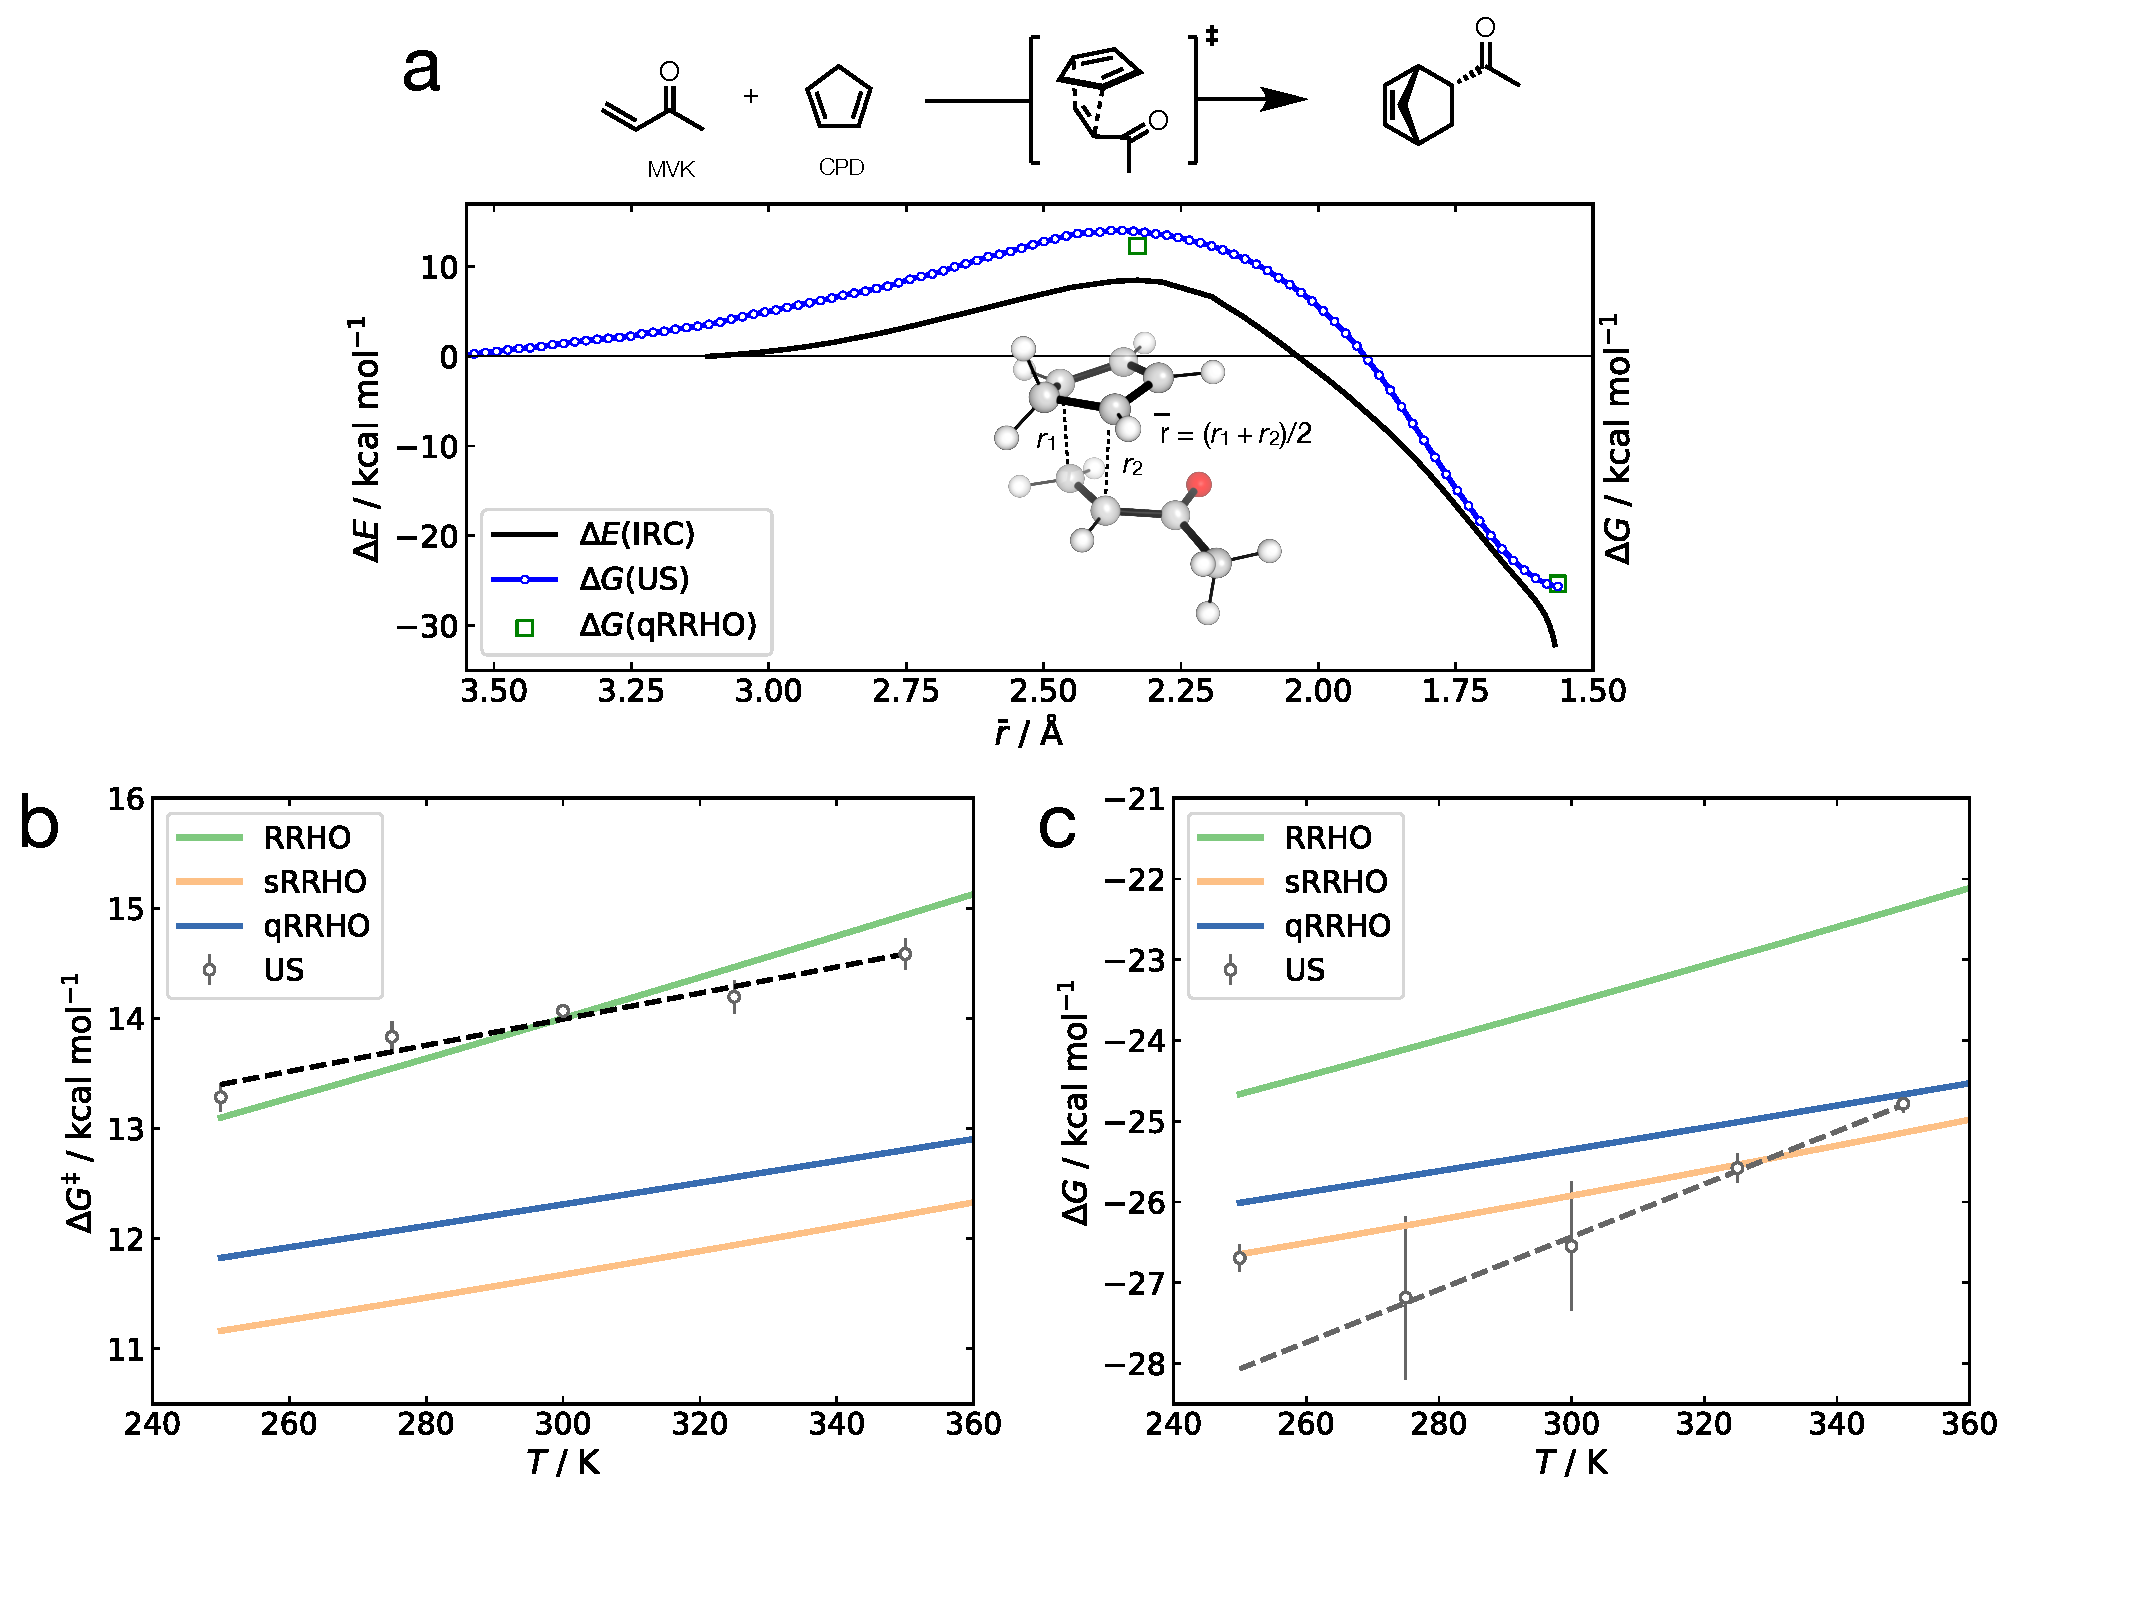
\includegraphics[width=13.0cm]{figX3}
	%\vspace{0.1cm}
	%\hrule
	%\vspace{0.1cm}
	\caption{(a) Convergence of the time gaps with the number of trajectories propagated via ACEs at different level of theory. Error is quoted as 2 σ. Dynamics propagated classically in the NVE ensemble initiated from TSs of corresponding functionals and initial velocities were obtained from Boltzmann distribution at 300 K. (b) Dependence of time gaps on type of dynamics with 200 trajectories. There are 4 types of dynamics: classical MD in the NVE ensemble and ring-polymer MD (RPMD) in the NVE ensemble with 16 beads initial from TS. The others are first equilibrated using constrained NVT RPMD (100 fs, applied harmonic potential with k = 5 eV/Å), then classical MD and RPMD in the NVE ensemble. All NVE propagated for 200 fs with a time step of 0.5 fs.}
	\label{fig::X4}
\end{figure*}

With a view to extend our initial GAP training methodology\cite{Young2021gap} into more complex systems and environments, we considered Diels-Alder (DA) reactions because of the available theoretical and experimental data,\cite{Black2012, Lording2020} and their prominence in chemical and biochemical contexts.\cite{Sato2021, MartCentelles2018, Briou2021} Initial efforts proved promising, with qualitatively reasonable reaction dynamics from [4+2] cycloaddition TSs for reactions between ethene + butadiene ({\bfseries{R1}}) and methyl-vinyl ketone + cyclopentadiene ({\bfseries{R2}}). Evaluating the quality of these potentials, however, revealed that they were not within the few $k_BT$ accuracy limit required for rate estimation or dynamic studies (see e.g., Fig. {\ref{fig::SX30}}a). A similarly complex but less exothermic reaction ({\ce{H3C}· + \ce{C3H8} $\rightarrow$ \ce{CH4} + ·\ce{CH(CH3)2}}) could be trained using the same strategy and hyperparameters (Fig. \ref{fig::SX30}b), suggesting that achieving 1 \kcal~accuracy within a 60 \kcal~energy window required for {\bfseries{R1}} is challenging for a GAP. Hyperparameter optimisation afforded an improvement, but at moderate computational cost ($\sim500$ configurations required for {\bfseries{R1}}). Specifically, reducing the regularisation, increasing the quality of the radial basis, and doubling the number of atomic environments considered in the training all improved the GAP (SI §\ref{section::SI_hyperparam_opt}). Systematic investigation of the effect of system size on the required number of reference evaluations suggests an approximate exponential scaling for a desired accuracy on the total energy (SI §\ref{section::SI_system_size}). Adopting new regression methods within the same training strategy (Fig. \ref{fig::X1}) shows that GAPs – even with hyperparameter tuning – are outperformed by both linear atomic cluster expansion (ACE\cite{Drautz2019}) and equivariant graph neural networks (NequIP\cite{Batzner2021}). Attempts to improve GAPs by training a component-wise potential separated over covalent bonds were unsuccessful (see SI §\ref{section::SI_ethene_butadiene_fragmentation}).


While rather different in philosophy, both ACE and NequIP provide MLPs that are similarly accurate for {\bfseries{R1}} (Fig. \ref{fig::X1}a, Fig. \ref{fig::SX23}).\footnote[4]{MLP training performed with \emph{ml-train}\cite{Young2021mlt} using \emph{QUIP},\cite{Csanyi_libAtoms_QUIP_2021} \emph{ACE},\cite{Ortner_ACE} \emph{ASE},\cite{HjorthLarsen2017} \emph{autodE},\cite{autodE} \emph{nequip}\cite{nequip_github} packages and ORCA\cite{Neese2017} for QM calculations. See SI for full methods.} Here, accuracy is based on deviations between true and predicted energies over independent DFT-MD trajectories propagated from the transition state (TS) to the reactant and product states. Previously, we have shown that a prospective validation strategy in the configuration space accessible to that MLP is essential to characterising `good’ MLPs.\cite{Young2021gap} However, here these potentials are stable within their the configuration space sampled from the TS by construction. This arises from the active learning strategy (Fig. \ref{fig::X1}, top) defining a stable potential where ten 1 ps trajectories can be propagated without encountering a configuration that is predicted to be $>2$ \kcal~(0.1 eV) above or below the true energy. Checking this criterion every MD step is too computationally intensive, thus stability is not guaranteed but empirically the criterion is sufficient to define stability within the maximum AL time (1 ps).


The data requirement to train a quality MLP for {\bfseries{R1}} is reduced upon GAP hyperparameter optimisation – even though the potential is more accurate – but is surpassed by the efficient ACE and NequIP potentials, both of which require only $\sim100$ training configurations ($n_\text{train}$, Fig. \ref{fig::X1}b). The total training time is maximal for the NequIP potential but is only $\sim1/2$ day (10 cores + 1 GPU) meaning it is suitable for rapidly developing bespoke MLPs. Note that the discrepancy between the MLPs in training time reduces with the system size, with reference energy and force evaluations dominating the computational time (for equally data efficient MLPs). The GAPs and ACE potential required just $5\pm2$ h of total training time on 10 CPU cores. The following sections will focus on ACE potentials for their slight advantage in computational cost.


As found for GAPs, re-evaluating energies and forces from AL configurations with a new reference method (aka. `uplifting’) reduces the computational cost associated with training WF-quality MLPs. For example, uplifting PBE0/DZ configurations to MP2/TZ affords an ACE potential within chemical accuracy to MP2-MD sampled configurations (Fig. \ref{fig::X1}c, DZ=double-$\zeta$ basis set, TZ=triple-$\zeta$).


Comparing the two-dimensional potential energy surface over the two forming C–C bonds, where all other degrees of freedom are free to relax, reveals that the ACE potential is smooth (as are the GAP and NequIP potentials, Fig. \ref{fig::SX25}) and accurate even in the extrapolation regime (Fig. \ref{fig::X1}d). Even where the closest configuration in the training data is 0.3 \AA~away in the forming bonds, the error is only a couple of \kcal~when AL is initiated at the TS ($r_1=r_2=2.30$ \AA).


Tangent to our goal of developing accurate MLPs for DA reactions, we found that GAP regularisation could be harnessed to reduce the computational cost of developing CCSD(T)-quality potentials (SI §S4). For simple molecules, MP2 forces are accurate to within $0.05$ eV \AA${}^{-1}$ of their CCSD(T) counterparts (Fig. \ref{fig::SX8}), thus within the `expected error’ (e.g. 0.1 eV \AA${}^{-1}$) of the GAP. This removes the requirement for numerical CCSD(T) gradients, while CUR\cite{Mahoney2009} selection can halve the dataset without compromising the accuracy (\tablename{ \ref{table::SX1}}). These effects can combine to afford a 100-fold reduction in the number of required CCSD(T) calculations.


Extending the reaction complexity, the ambimodal reaction between tropone and cyclohepatriene ({\bfseries{R3}}) is capable of forming three distinct products from a single TS (Fig. \ref{fig::X2}, top).\cite{Jamieson2021} Training an ACE potential from the TS ({\bfseries{R3$_\text{TS1}$}}) generated $\sim450$ configurations using standard AL with sampling in the reactant and product regions of 2 of the 3 products. However, despite propagating ACE-MD at 500 K, the Cope product ({\bfseries{R3$_\text{P3}$}}) was not present in the training data, making it unsuitable for running dynamics to elucidate the product ratio. Only when the TS that leads directly to {\bfseries{R3$_\text{P3}$}} is included as an AL starting configuration is the training data sufficiently complete. This highlights the importance of considering relevant points close in energy (4.4 \kcal, ref. \citenum{Jamieson2021}) when training MLPs, that may not be obtained using automated sampling methods. For {\bfseries{R3}} the ACE required $\sim 2$ days of AL and -- in contrast to simple systems -- we found is was not possible use a distance criteria to select configurations, with no {\bfseries{R3$_\text{P1}$}} sampled in training (see §S\ref{section::SI_AL_strategies}).


Employing this MLP to propagate dynamics enables unique observations compared to the most common DFT-MD approach. Specifically, because each 1 ps trajectory takes only a couple of minutes to calculate, the product distribution can be converged with respect to the number of trajectories (Fig. \ref{fig::X2}a). Using only 100 trajectories affords an error ($2\sigma$, 95\% confidence) of 10\% for product {\bfseries{R3$_\text{P2}$}}, which may, or may not, be sufficient for experimental comparison.


The inference efficiency also enables quantum dynamics to be propagated, which otherwise be too computationally demanding. Interestingly, we find that initiating ring-polymer molecular dynamics (RPMD)\cite{Habershon2013} without equilibrating the ring polymer leads to very similar product ratios to the classical dynamics, despite the zero-point energy being included as the ring polymer `swells’. Equilibrating the system at the TS in the NVT ensemble with weak restraints (1 eV \AA$^{-1}$, $\sim0.5$ \kcal~additional ZPE) prior to NVE downhill dynamics affords almost double the proportion of {\bfseries{R3$_\text{P1}$}} and the formation of 10 as 1 \% of the total product distribution. Training an MLP potential uniquely allows for the 100-fold more expensive simulations to be performed and the effect of ZPE (without leakage\cite{Lee2018}) and tunnelling accounted for. Note that the equilibrated quantum dynamics are required to for correct dynamics\cite{Liu2019} thus the right most distribution in Fig. \ref{fig::X2}b should be considered the benchmark.


With MLP uplifts to different levels of theory affordable, the effect of methodology on product distributions can be evaluated (100s CPUh vs. $>200,000$ CPUh for the data in Fig. \ref{fig::SX31}).  Interestingly, we find that some levels require a few iterations of AL from their TSs if the configuration space overlap with the training level is poor. For example, B3LYP distributions are unchanged on additional AL, while M06-2X affords $\sim10$\% more product {\bfseries{R3$_\text{P2}$}} upon a further five AL iterations. Product distributions vary considerably between functionals, with the major state varying from the reactant to {\bfseries{R3$_\text{P2}$}} and the proportion of {\bfseries{R3$_\text{P1}$}} varying from 1 to 10\% (see Fig. \ref{fig::SX31}). Downhill AIMD-derived product distributions should therefore consider the PES influence on the results more so than the type of dynamics (classical vs. quantum).


Herein, we applied the ACE potentials to propagate molecular dynamics to investigate the reactions {\bfseries{R2}} initiated from the TS until either the cycloadduct is formed (the two forming C-C bond lengths < 1.6 Å), or the reactants are separated (the two forming C-C bond lengths > 3.0 Å) with a maximum simulation time of 500 fs (Figures X). The time gaps, denoted as the time difference between formations of two C-C $\sigma$ bonds, can be were around 20 fs for PBE0 and $\omega$B97-XD and 10 fs for M06-2X level of theory on average. Although longer time gaps for PBE0 and $\omega$B97-XD functionals, they are still smaller than 30 fs, the C-C vibrational period, and can be regarded as dynamically concert. Quantum effects on this reaction were also explored by propagting the RPMD at $\omega$B97-XD due to its ability of calculating geometries and energies of asynchronous Diels-Alder reaction. (Detail discussion of RPMD will be added after finishing running other 300 trajectories).


Obtaining free energies from absolute estimates in the rigid-rotor harmonic oscillator (RRHO) method is deficient in the low frequency regime.\cite{Liu2017} To investigate the effect of different static approaches (RRHO, sRRHO,\cite{Ribeiro2011} qRRHO\cite{Grimme2012}) we trained an ACE potential for {\bfseries{R2}} and compared free energy differences to classical umbrella sampling (US, Fig. \ref{fig::X3}). Reactive simulations totalling 1.5 ns would be unobtainable with DFT-MD. Note the sampling in the product state at 250 K is insufficiently complete, thus is excluded from the linear fit. The anharmonic effects at the reactant complex are significant, leading to a spread of 2 \kcal~within the static methods, while the US correctly captures those effects but fails to treat any nuclear quantum effects. Therefore, for DA reactions any calculated free energies should include a few \kcal~error bar, even with perfect electronic energies.

Finally, we considered the DA reaction between cyclopentadiene and acetylene ({\bfseries{R4}}) for which experimental gas-phase kinetic data are available.\cite{Walsh1975} Classical umbrella sampling from an MLP is sufficient to obtain quantitative accuracy (Table \ref{tbl::X1}). While the potential fitting is completely automated, determining an appropriate QM reference method and US require human intervention. Future work will address these points and approach an automated prediction of activation entropies and enthalpies. Nevertheless, these data show that free energies with associated errors, and treatment of anharmonic effects without \emph{ad-hoc} corrections, are now achievable.


\begin{table}[h]
	\small
	\caption{\ Activation parameters for {\bfseries{R4}} obtained from ACE umbrella sampling (US). See SI §S\ref{section::SI_R4} for details. Standard error in the last digit is quoted in parenthesis.}
	\label{tbl::X1}
	\vspace{-0.2cm}
	\renewcommand{\arraystretch}{1.4}
	\begin{tabular*}{0.48\textwidth}{@{\extracolsep{\fill}}lll}
		\hline
		 & $\Delta H^\ddagger$ / \kcal & $\Delta S^\ddagger$ / cal K${}^{-1}$ mol$^{-1}$ \\
		\hline
		US & $20(3)$ & $-32(8)$ \\
		expt.\cite{Walsh1975} & $21.9(1)$ & $-37.3(2)$ \\
		\hline
	\end{tabular*}
\end{table}


% DSDPBE -B86 error: 0.1371612392 eV = 3.1 kcal mol-1 on the B2PLYP surface


\vspace{0.2cm}
The comparison of three machine learned potential (MLP) methods suggests that the atomic cluster expansion (ACE) framework is efficient and accurate for modelling highly-exothermic and modestly complex ($\sim 50$ atoms) Diels-Alder reactions. Using the freely available automated fitting code \emph{ml-train}\cite{Young2021mlt} several ACE potentials were fitted and consistently achieve \emph{chemical accuracy} ($\pm$ 1 \kcal) to the ground-truth surface. Product distributions obtained from DFT-MD trajectories from ambimodal transition states are strongly depending on the reference method, are not strongly dependent on propagating quantum dynamics but do require at least several hundred trajectories to converge. Static quantum mechanical free energy methods vary by several \kcal~in barrier and reaction energies, while umbrella sampling straddles the range. Comparison of MLP-derived and experimental free energy differences suggest that classical methods are sufficient for quantitative comparison for these systems. These insights would not be possible without having trained accurate and efficient MLPs. Advancements in reference methods are needed to obtain accurate potentials within a day without a proceeding benchmark study, however we are confident this will enable routine development of chemically accurate MLPs.


\section*{Conflicts of interest}
There are no conflicts to declare.

\section*{Acknowledgements}
TJW acknowledges the EPSRC Centre for Doctoral Theory and Modelling in Chemical Sciences (EP/L015722/1) and TAY the EPSRC impact acceleration account (IAA) grant (EP/R511742/1). 


%%%END OF MAIN TEXT%%%

%  For footnotes in the main text of the article please number the footnotes to avoid duplicate symbols. e.g.  \footnote[num]{your text} the corresponding author \ast counts as footnote 1, ESI as footnote 2, e.g. if there is no ESI, please start at [num]=[2], if ESI is cited in the title please start at [num]=[3] etc. Please also cite the ESI within the main body of the text using \dag.

% The \balance command can be used to balance the columns on the final page if desired. It should be placed anywhere within the first column of the last page.

% \balance

% If notes are included in your references you can change the title from 'References' to 'Notes and references' using the following command:
% \renewcommand\refname{Notes and references}

%%%REFERENCES%%%
\scriptsize{
\bibliography{refs} %You need to replace "rsc" on this line with the name of your .bib file
\bibliographystyle{rsc} } %the RSC's .bst file

\end{document}
